%!TEX root = main.tex
% a Identify different factors explaining (causing) the variance in the metric,



We recall from our previous work the definition of the metric used to quantify botnet infection (BNI) problem, namely \textit{BNI attempts} which measures the number of attacks executed daily. In figure ~\ref{fig:isp_legend_area}, we show the output of this metric for different Autonomous Systems (AS) ran by ISPs. It is normalized by the address space of each AS, however, in order to explain the variation between AS\/ISP's in this section we identify, analyze and statistically describe the factors behind the variance of the metric defined before.

\subsection{Identifying the underlying factors}
To successfully identify the factors behind the BNI attempts variance first we would like to give an intuition of how does this security issue propagates within a network. A botnet is more likely to try more infection attempts if a it is either active, big or both. The likelihood infection of a potential zombie machine is mainly influenced by the following two factors: how close the potential new member is (w.r.t. euclidean or geodesic~\cite{geodesic} distance) and how secure is the his system.
The former factor, the distance between a zombie machine and a potential new member of the botnet might be represented by the geographic distance or the logical distance within a network topology, i.e. the type of network in which the zombie machine is connected (Wifi public hot-spot, home network, enterprise network), the Internet penetration in the country or region (High Internet penetration rate may lead to club effect behaviors~\cite{club_effects}).

The latter factor, the security of the potential zombie machine might depends on different software and hardware variables, i.e. operative system (OS) and application vulnerabilities, software updates (issued patches of known vulnerabilities for a particular version), hardware reliability (backdoor presence), user awareness.
%TODO normalize data by address space

\begin{figure}[h]
     \caption{Infection attempts per day in different AS of the ISPs normalized by address space and multiplied by $10^9$}
     \label{fig:isp_legend_area}
    \centering
    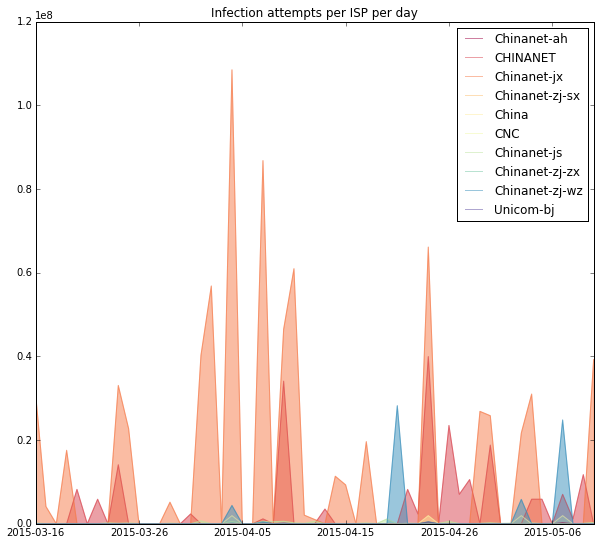
\includegraphics[width=\linewidth]{images/isp_legend_area_norm}
\end{figure}

\subsection{Statistical analysis of the underlying factors}
In figure~\ref{fig:os_distribution} we show the distribution of OS along different AS, as we might the most common OS in every AS is \textit{Windows 2000}, however, this OS is far to be the most deployed OS as we show in figure~\ref{fig:os_pen} and in \cite{os_pen} at the end 2014 \textit{Windows 2000} only had less than the 0.05\%.
On the other hand, we would like to analyze the number of vulnerabilities of different software vendors, in figure~\ref{fig:vul_ven} we can see the to number of vulnerabilities in the top 50 products of each vendor, again Windows 2000 is not in the most vulnerable systems, however, when we look at the details we can see that 42\% of all the vulnerabilities in this OS are of the Code Execution (CE)type and there is at least 16 exploits published.


\begin{figure}[h]
     \caption{Number of vulnerabilities per vendor~\cite{vul_ven}}
     \label{fig:vul_ven}
    \centering
    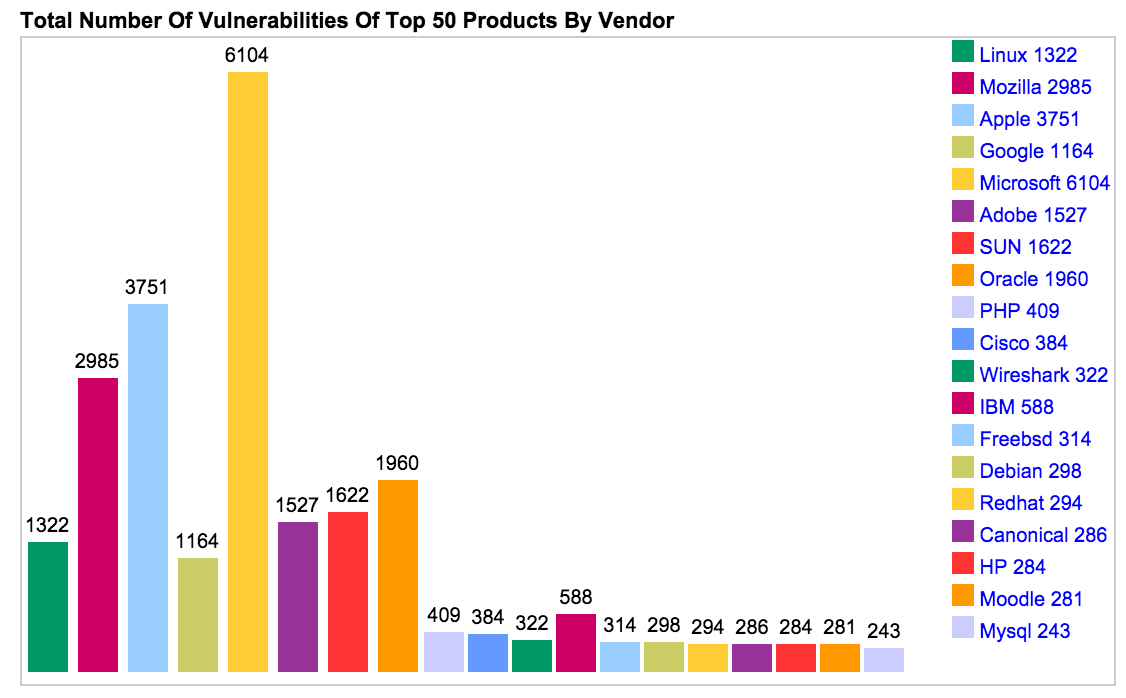
\includegraphics[width=\linewidth]{images/vul_ven}
\end{figure}

\begin{figure}[h]
     \caption{OS market share}
     \label{fig:os_pen}
    \centering
    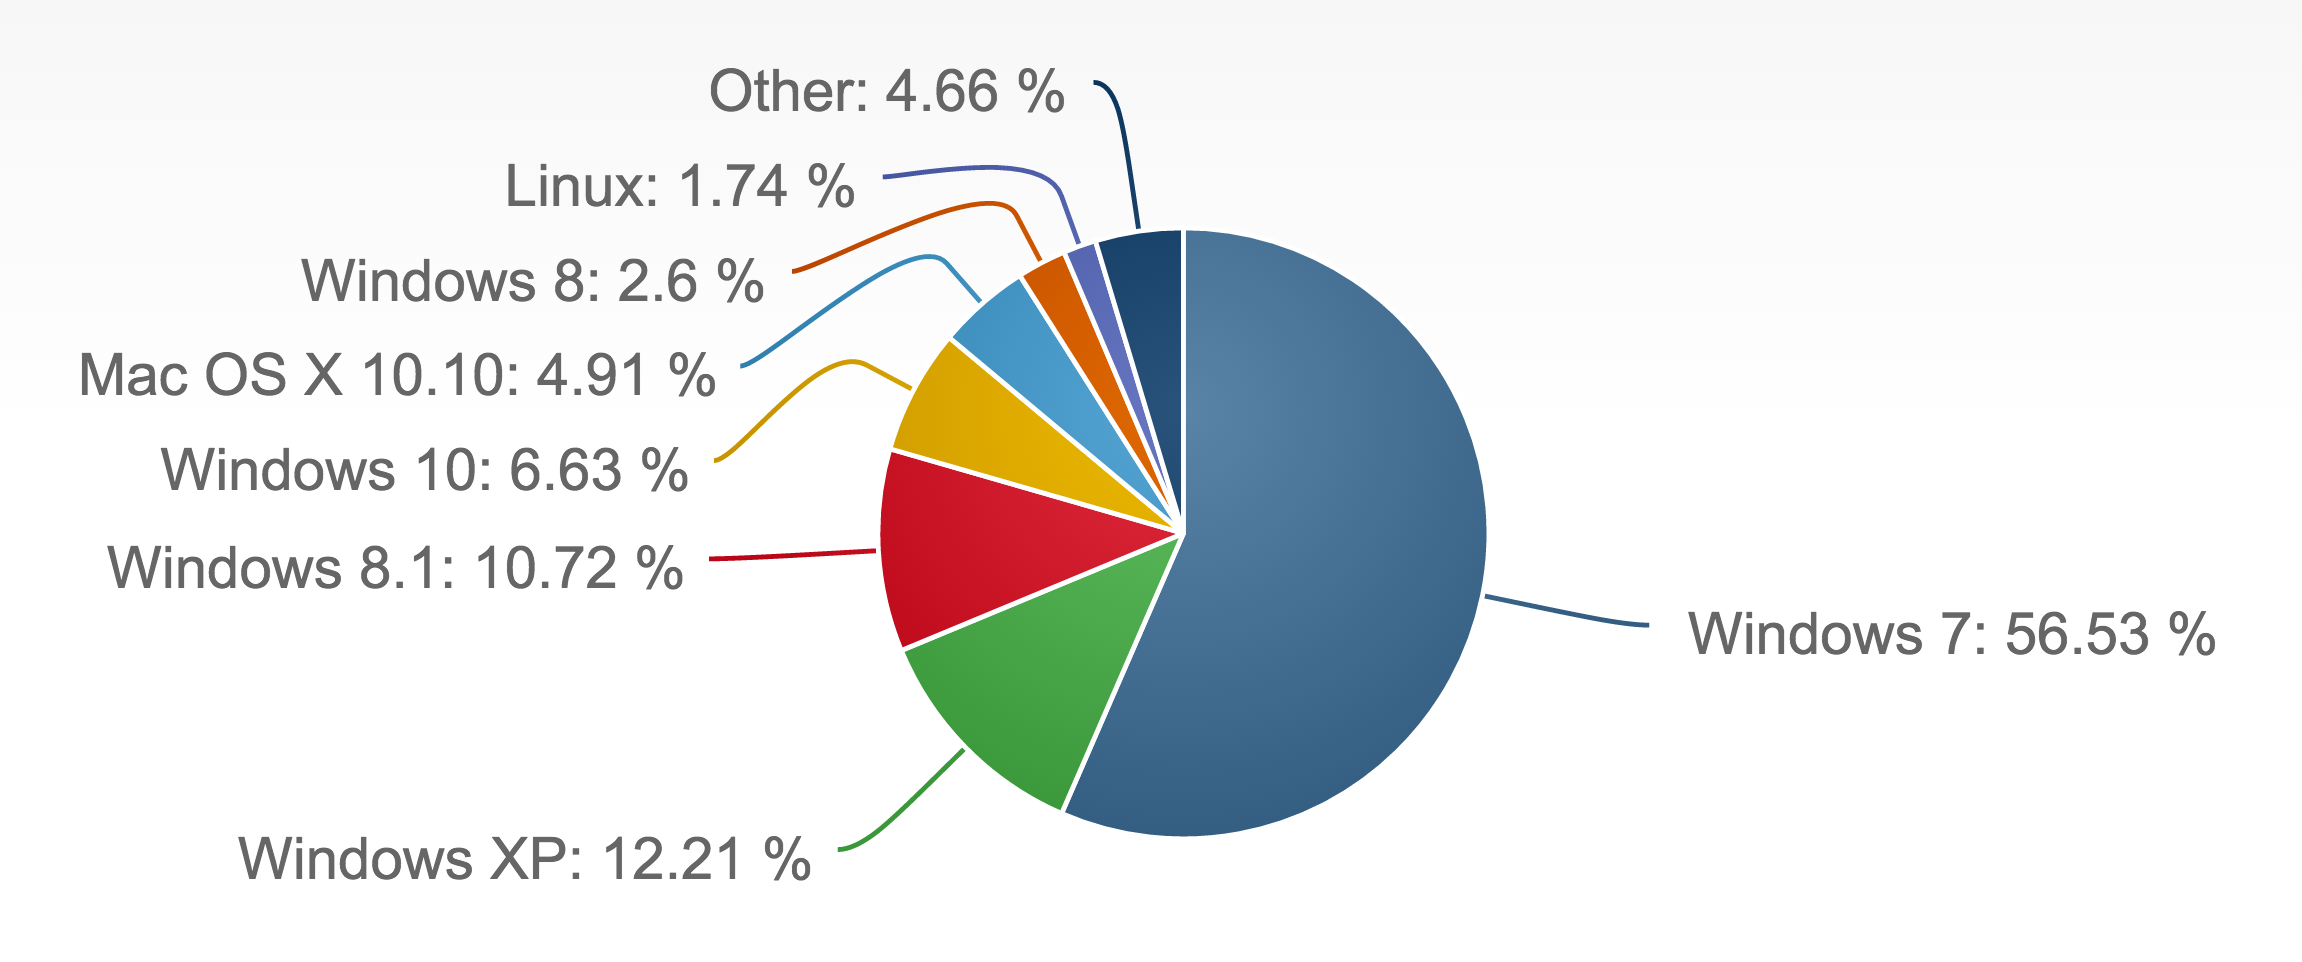
\includegraphics[width=\linewidth]{images/os_pen}
\end{figure}
% \subsubsection{OS}

\begin{figure}[h]
     \caption{OS distribution among the more active ISP's ASs}
     \label{fig:os_distribution}
    \centering
    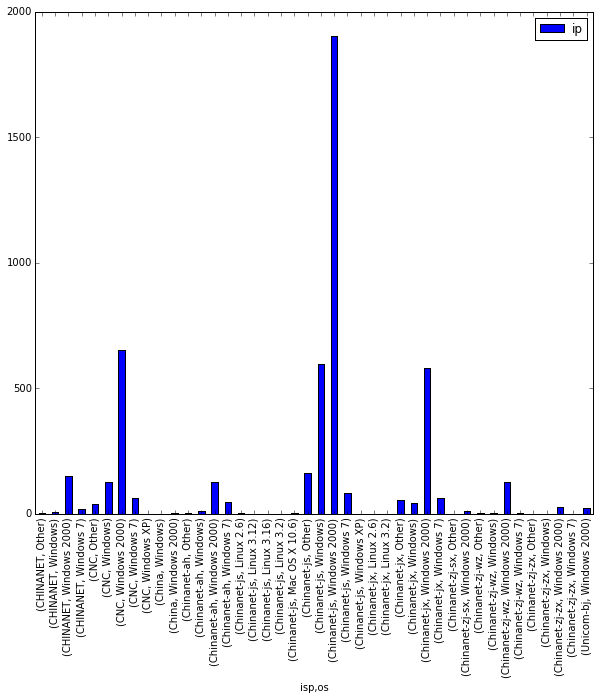
\includegraphics[width=\linewidth]{images/os_isp}
\end{figure}
% section explaining_the_variance_in_botnet_infection_ (end)
